% !TeX spellcheck = en_US

\newcommand{\resultsPlotWidthScale}{1}
\newcommand{\resultsFigureWidthScale}{0.8}

\chapter{Results}
\label{chap:results}

\section{\ref{PS:Q:Feasibility}}
\label{sec:exp:feasibility}
Presented in \cref{fig:graphicalInterface} is shown a screenshot of the graphical interface while the decentralized solution is running 5 turbines.
The global setpoint for power production is at 2000, illustrated by the red line and global power production is illustrated by the black line.
The blue line illustrates the maximum available power production for the wind farm while the lines in the bottom around 400 is the power production of each individual turbine.

\begin{figure} [!h]
	\centering
	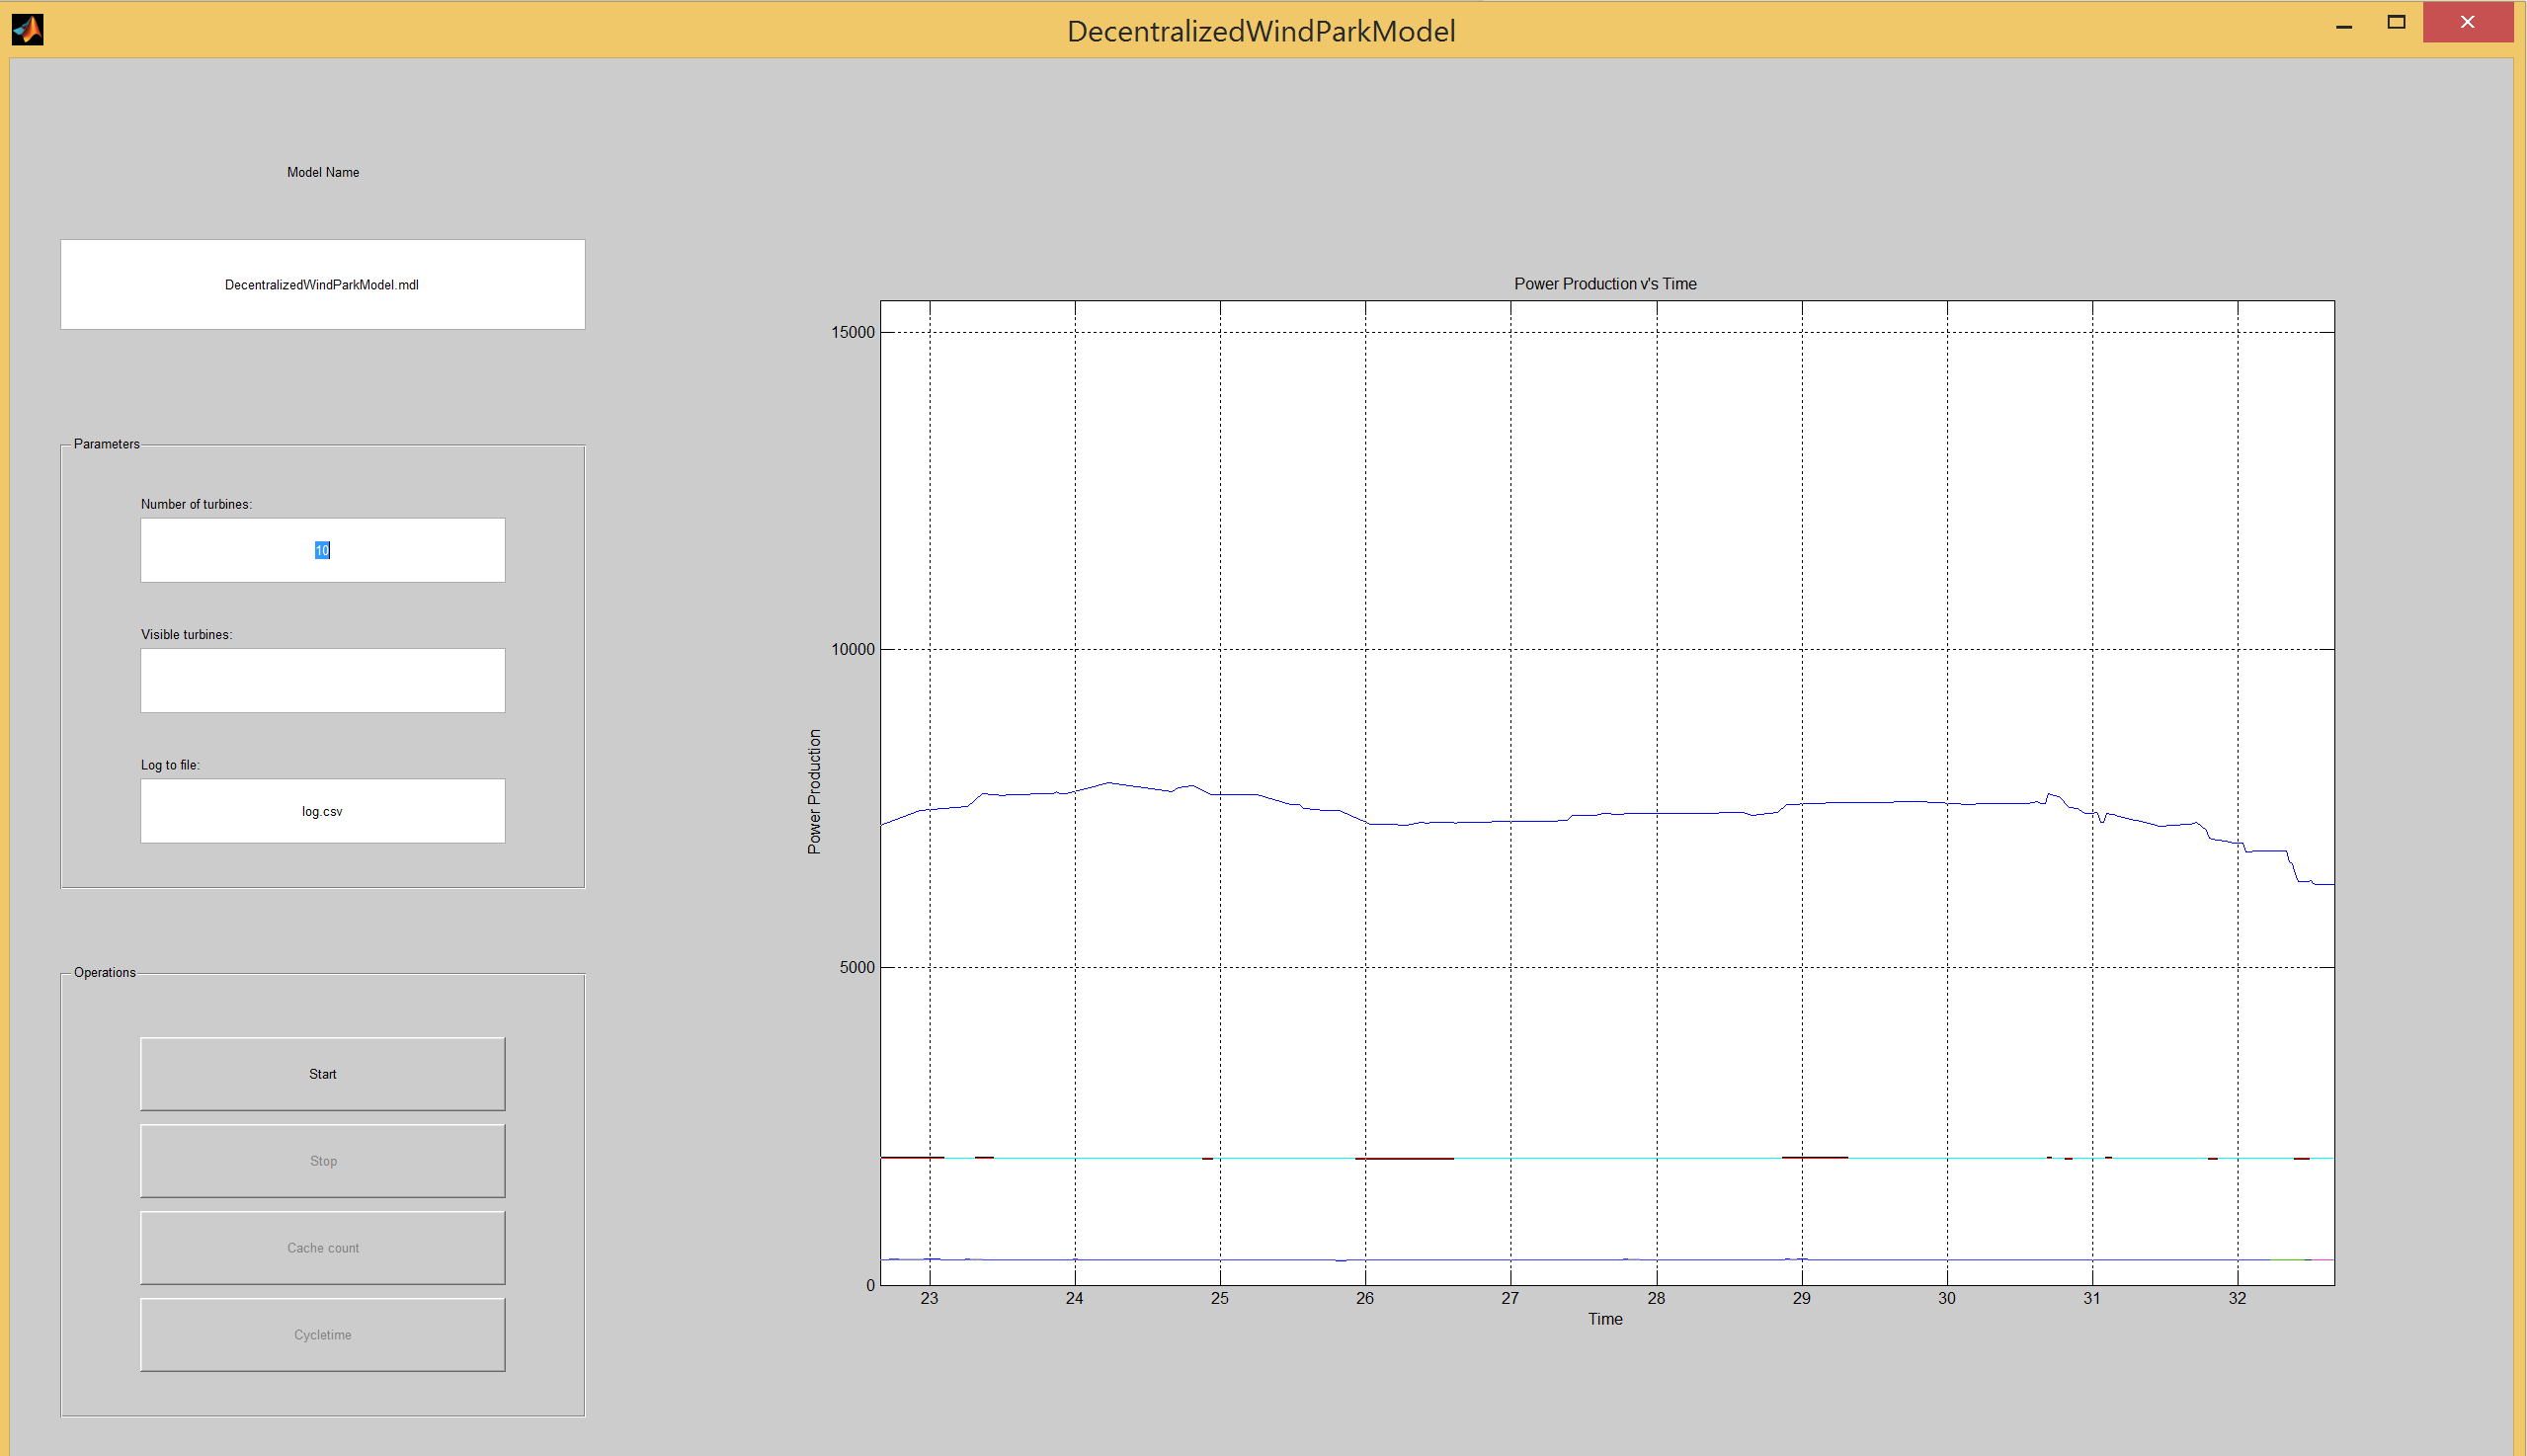
\includegraphics[width=\resultsFigureWidthScale\textwidth]{gui.png} 
	\captionsetup{format=plain,font=footnotesize,labelfont={bf,defaultCapFont},labelsep=quad,singlelinecheck=no}
	\caption[Graphical interface running 5 turbines]{
		\label{fig:graphicalInterface} 
		\footnotesize{%
			Graphical interface running 5 turbines.
		}
	}
\end{figure}


\section{\ref{PS:Q:Availability}}\FloatBarrier

The plots in \cref{fig:exp:availability_kill15,fig:exp:availability_kill10,fig:exp:availability_kill5,fig:exp:availability_kill1} show how the decentralized solution reacts when killing 1, 5, 10 and 15 turbines. To begin with there are 30 turbines, the setpoint is set to 2,000 for all setups except for when killing only one turbine(\cref{fig:exp:availability_kill1}) it was set to 20,000. This was done so that it was possible to visually verify that the turbines reacted.
The turbines are all running with a cycle time of 20 ms.

\begin{figure}
	\centering
	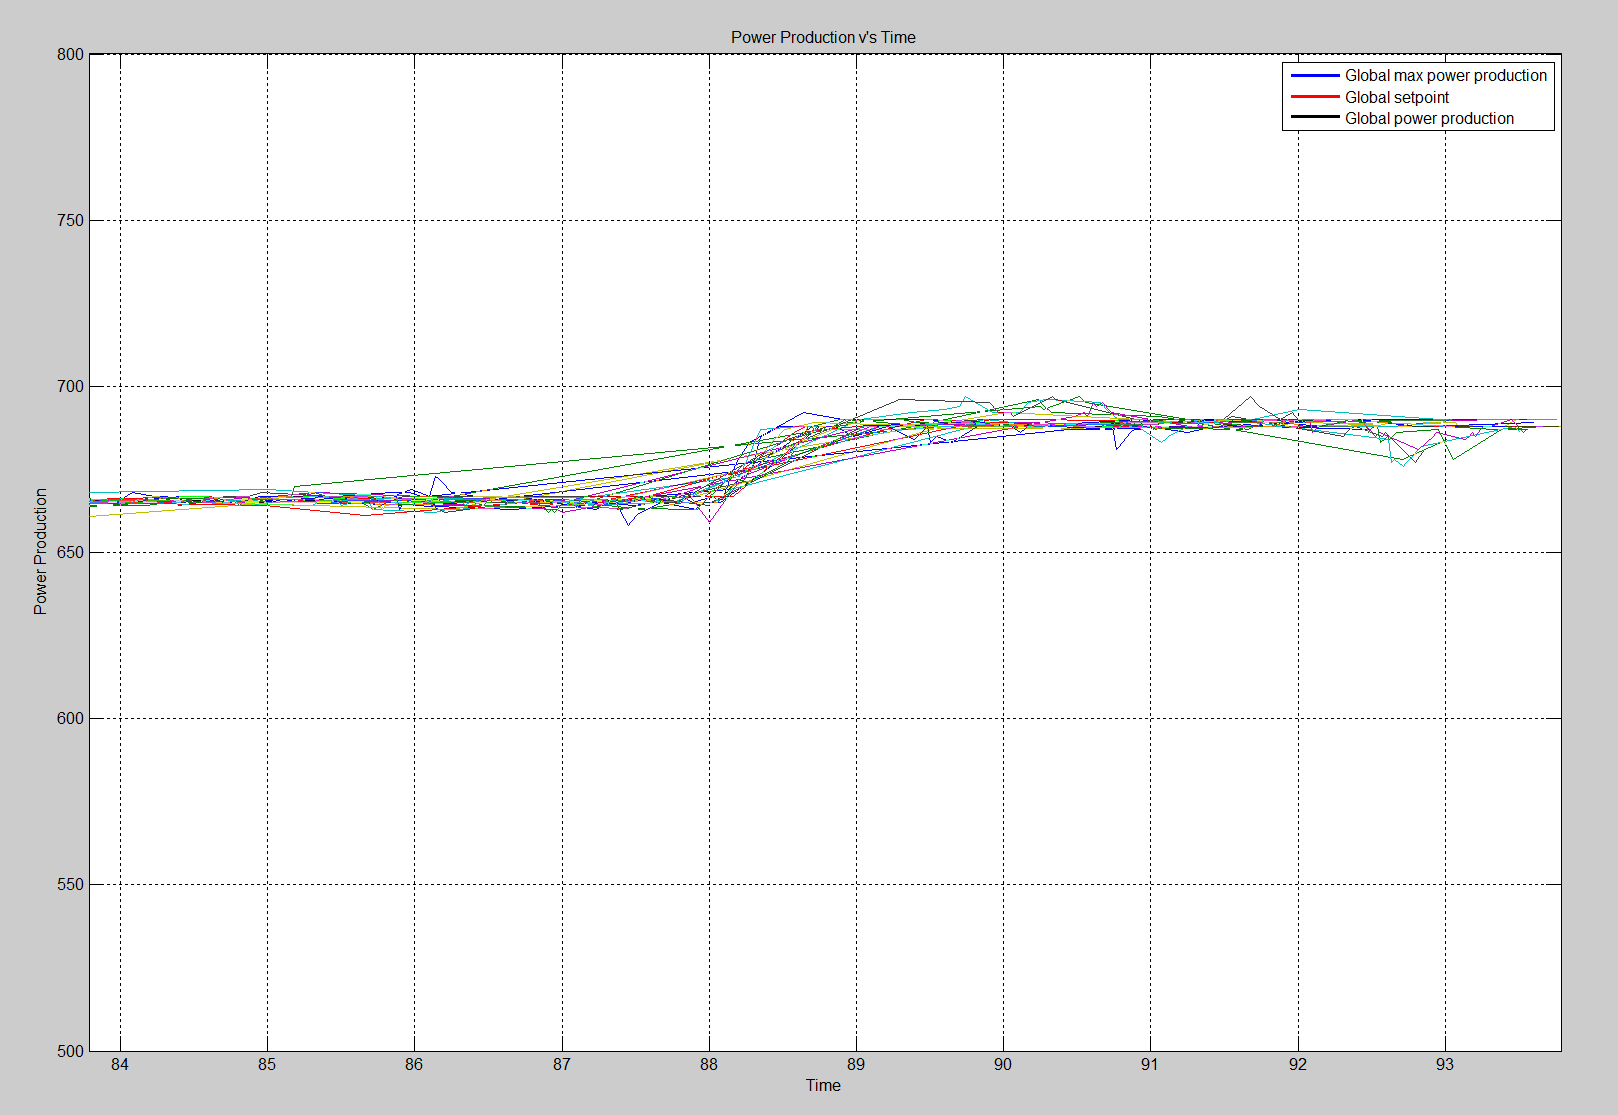
\includegraphics[width=\resultsFigureWidthScale\textwidth]{figures/Results/availabilitytest30-29_setpoint_20000.PNG}
	\caption{Availability test kill 1 out of 30 turbines}
	\label{fig:exp:availability_kill1}
\end{figure}

\begin{figure}
	\centering
	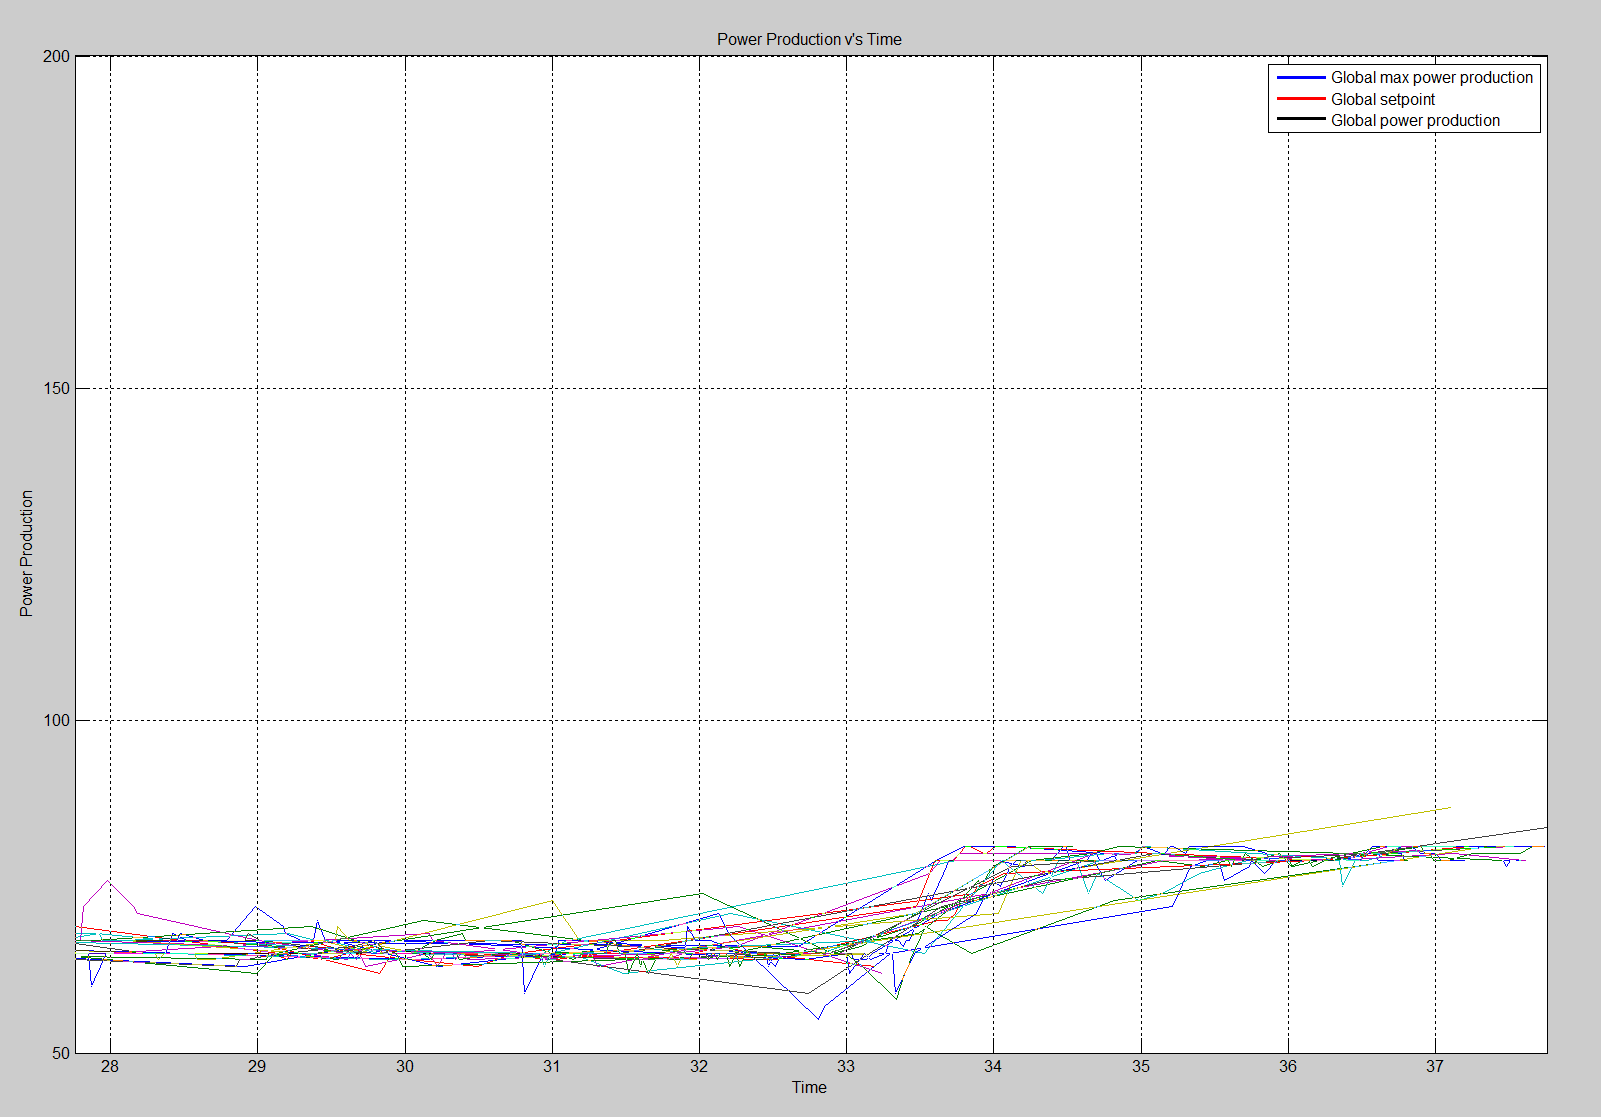
\includegraphics[width=\resultsFigureWidthScale\textwidth]{figures/Results/availabilitytest30-25_setpoint_2000.PNG}
	\caption{Availability test kill 5 out of 30 turbines}
	\label{fig:exp:availability_kill5}
\end{figure}

\begin{figure}
	\centering
	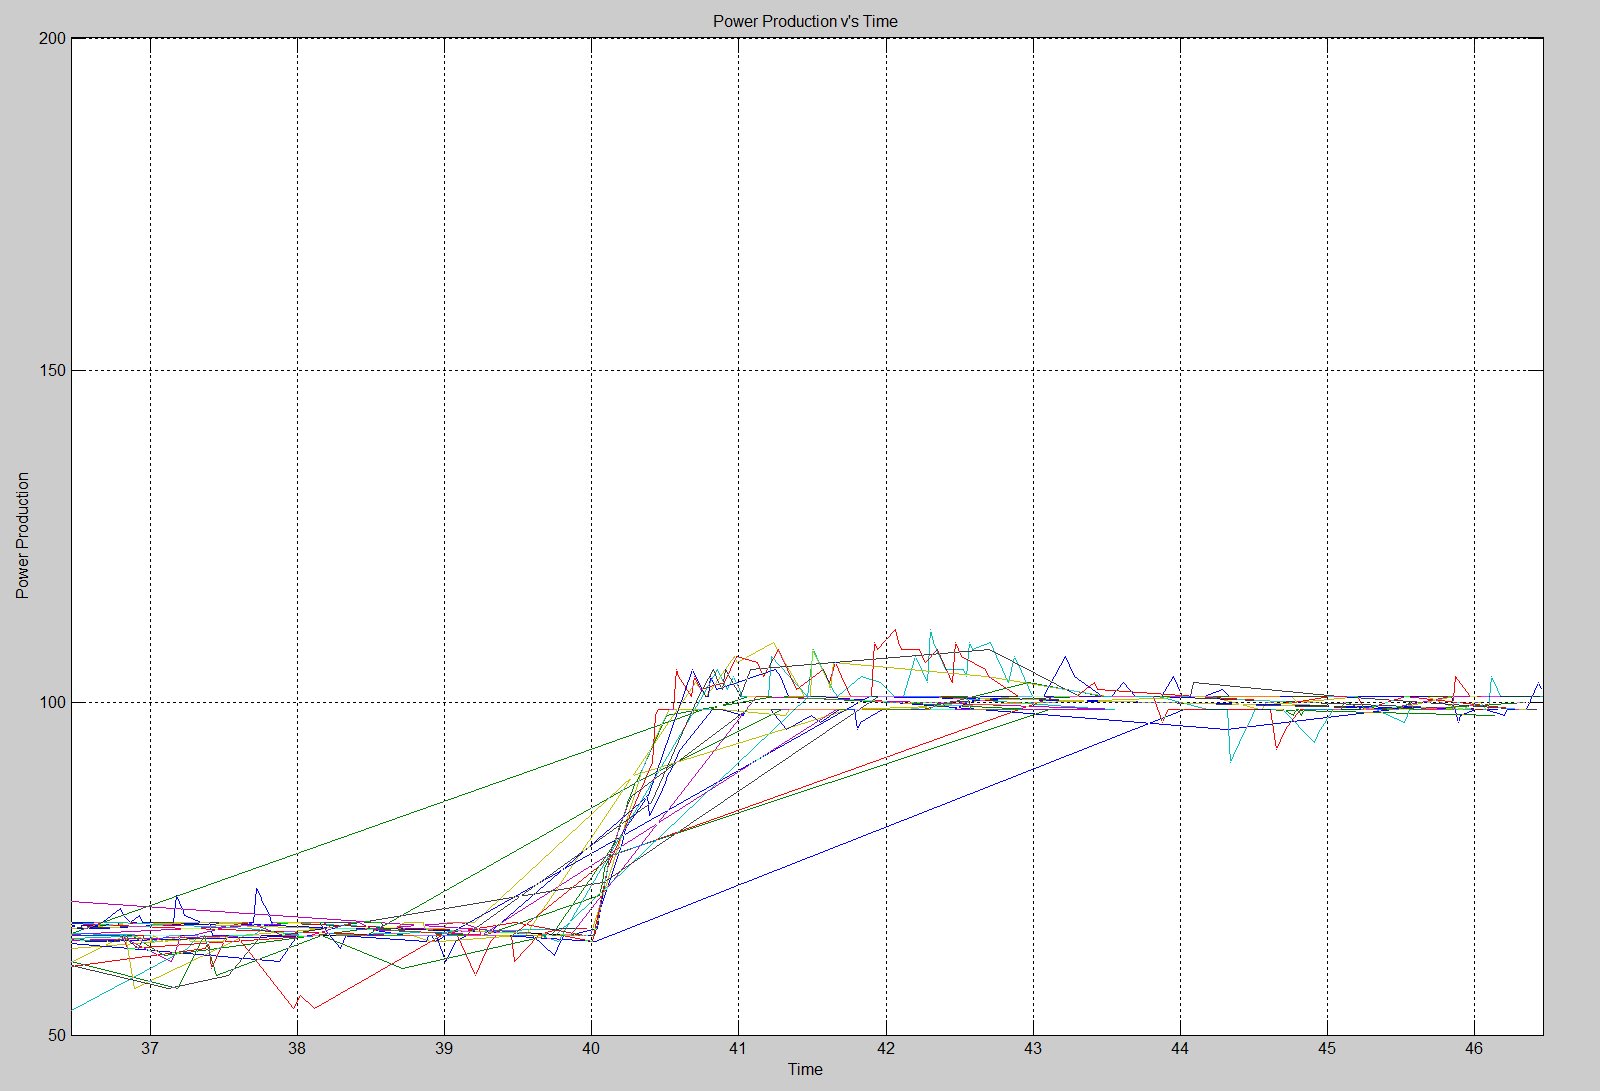
\includegraphics[width=\resultsFigureWidthScale\textwidth]{figures/Results/availabilitytest30-20_setpoint_2000.PNG}
	\caption{Availability test kill 10 out of 30 turbines}
	\label{fig:exp:availability_kill10}
\end{figure}

\begin{figure}
	\centering
	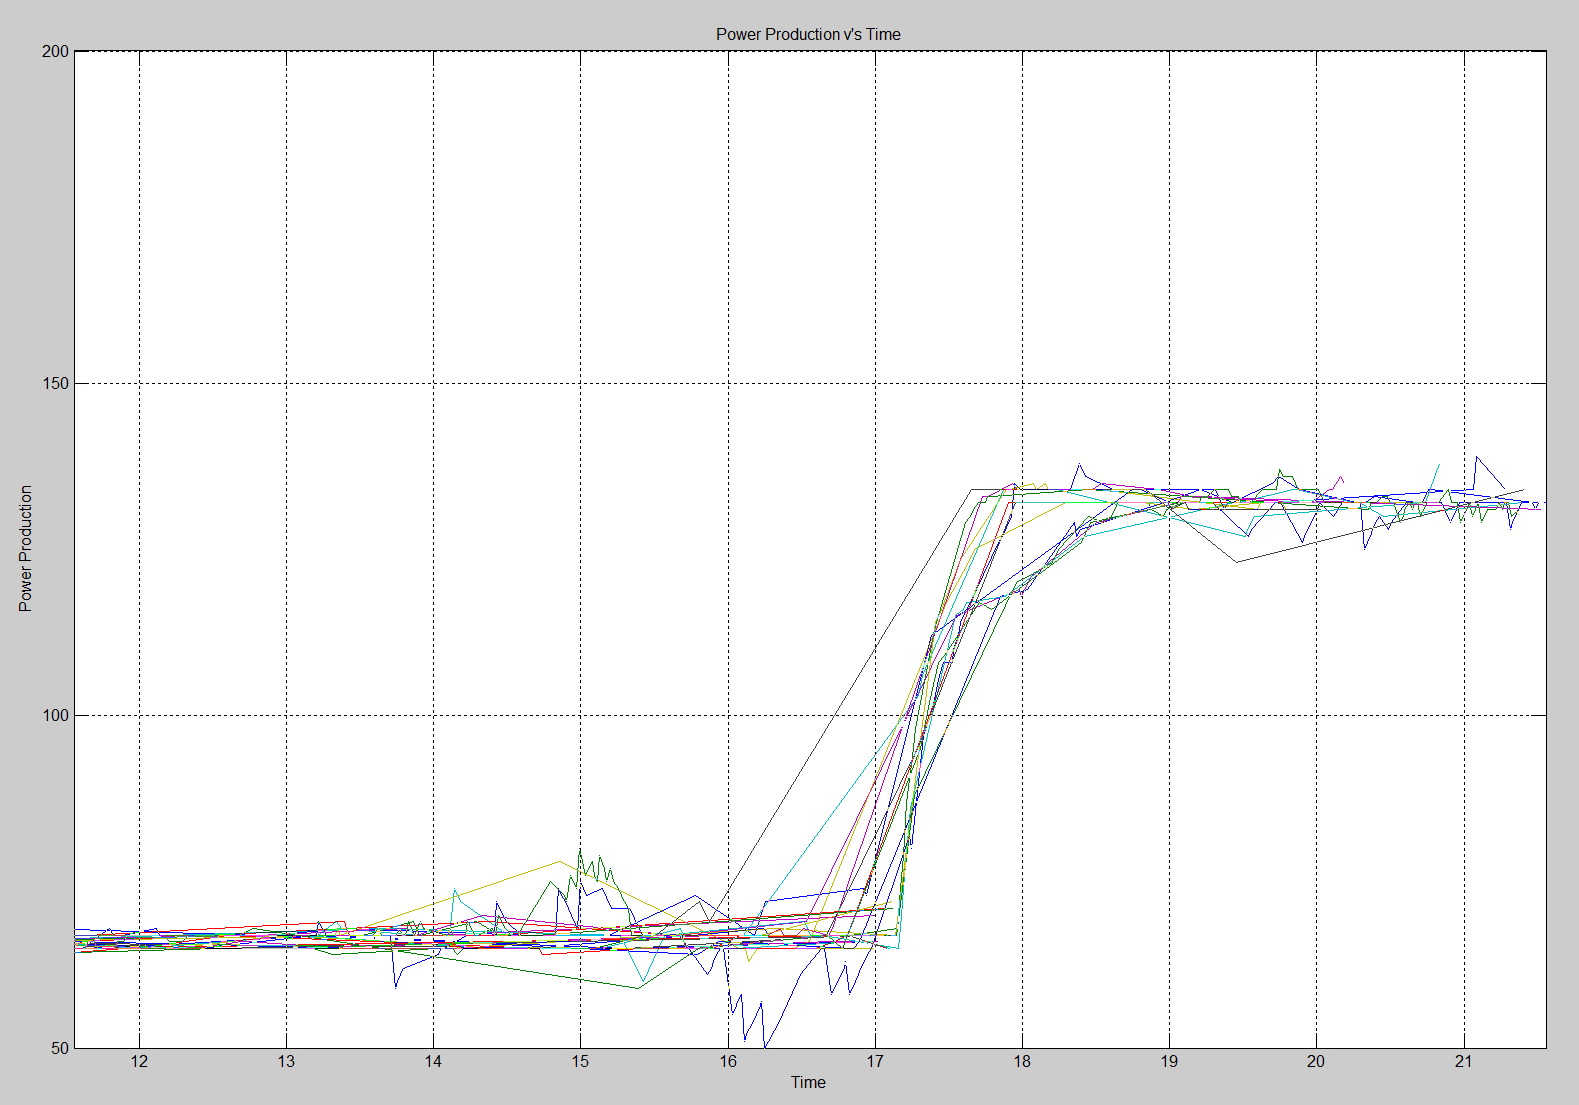
\includegraphics[width=\resultsFigureWidthScale\textwidth]{figures/Results/availabilitytest30-15_setpoint_2000.PNG}
	\caption{Availability test kill 15 out of 30 turbines}
	\label{fig:exp:availability_kill15}
\end{figure}

\clearpage
\section{\ref{PS:Q:Performance}}\FloatBarrier
\label{sec:exp:performance}
The cycle times are calculated as the difference between the receive timestamp of the oldest turbine state package and a timestamp right after the new turbine state has been sent and the turbines setpoint has been set.
The regulation cycle time with variating number of turbines are done with box plots and a line. The box plots whiskers show the extreme values max and min, the top and bottom of the box show the upper and lower quartile of the data, and the center line shows the median. The median is further highlighted by a line.

\subsection{\nameref{subsec:Exper:perfom:1}}

The results of one of the \nameref{sec:Exper:perfom} experiments plotted are plotted in \cref{fig:exp:decen:sleep,fig:exp:decen:sleep-cache}.
The experiment where performed with a variating number of internal wait times.

\begin{figure}[h!]
	\centering
	\begin{tikzpicture}
\begin{axis}
[
width=\resultsFigureWidthScale\textwidth,
axis y line*=left,
xlabel=Sleeptime (ms),
ylabel=Regulation cycle time (ms),
ymin = 0,
xtick={1, 2, 3, 4, 5, 6, 7, 8, 9},
xticklabels={10, 15, 20, 25, 30, 35, 40, 45, 50},
boxplot/draw direction=y
]

%% /home/stefan/work/TestResults/Test6_Decentralized_12-7-2014_1327/nCycleTime/DecentralizedLog1.csv
\buildBoxPlot{10.578002}{15.286001}{9.942}{148.911}{0.415002}

%% /home/stefan/work/TestResults/Test6_Decentralized_12-7-2014_1327/nCycleTime/DecentralizedLog2.csv
\buildBoxPlot{15.026002}{15.383002}{14.312002}{26.729001}{1.379}

%% /home/stefan/work/TestResults/Test6_Decentralized_12-7-2014_1327/nCycleTime/DecentralizedLog3.csv
\buildBoxPlot{19.926}{20.380001}{18.979001}{29.932002}{0.435}

%% /home/stefan/work/TestResults/Test6_Decentralized_12-7-2014_1327/nCycleTime/DecentralizedLog4.csv
\buildBoxPlot{25.079001}{25.322}{24.637001}{32.794001}{12.225002}

%% /home/stefan/work/TestResults/Test6_Decentralized_12-7-2014_1327/nCycleTime/DecentralizedLog5.csv
\buildBoxPlot{30.099}{30.363}{29.565001}{42.436}{4.466}

%% /home/stefan/work/TestResults/Test6_Decentralized_12-7-2014_1327/nCycleTime/DecentralizedLog6.csv
\buildBoxPlot{35.153001}{35.328002}{34.853001}{45.836001}{10.347}

%% /home/stefan/work/TestResults/Test6_Decentralized_12-7-2014_1327/nCycleTime/DecentralizedLog7.csv
\buildBoxPlot{40.157001}{40.434001}{39.626}{58.338001}{6.398001}

%% /home/stefan/work/TestResults/Test6_Decentralized_12-7-2014_1327/nCycleTime/DecentralizedLog8.csv
\buildBoxPlot{45.185}{45.330001}{44.928002}{50.089}{29.313}

%% /home/stefan/work/TestResults/Test6_Decentralized_12-7-2014_1327/nCycleTime/DecentralizedLog9.csv
\buildBoxPlot{49.958002}{50.391001}{49.019}{64.611002}{4.846}


\addplot[thick, red!70] coordinates {
	(1 ,10.578002)
	(2 ,15.026002)
	(3 ,19.926)
	(4 ,25.079001)
	(5 ,30.099)
	(6 ,35.153001)
	(7 ,40.157001)
	(8 ,45.185)
	(9 ,49.958002)
	
};

\end{axis}
\end{tikzpicture}

	\caption{Decentralized solution with variable wait time cycle time experiment}
	\label{fig:exp:decen:sleep}
\end{figure}

\Cref{fig:exp:decen:sleep} show the that the regulation cycle times and wait times are linearly Dependant on each other, the maximum value with wait time 10 is outside the boundaries of the plot but is calculated to 148.91 ms The upper and lower quartile are close together the exception is the 10 ms wait time sample, the maximum being the 20 ms wait time having a difference of 1.401 ms between upper and lower quantile and the minimum being 45 ms wait time with a difference of 0.402 ms The maximum values again with the exception of the 10 ms wait time sample follow the median values, the minimum values are able to reach low regulation cycle times much lower than the wait time used in the experiment.

\begin{figure}[h!]
	\centering
	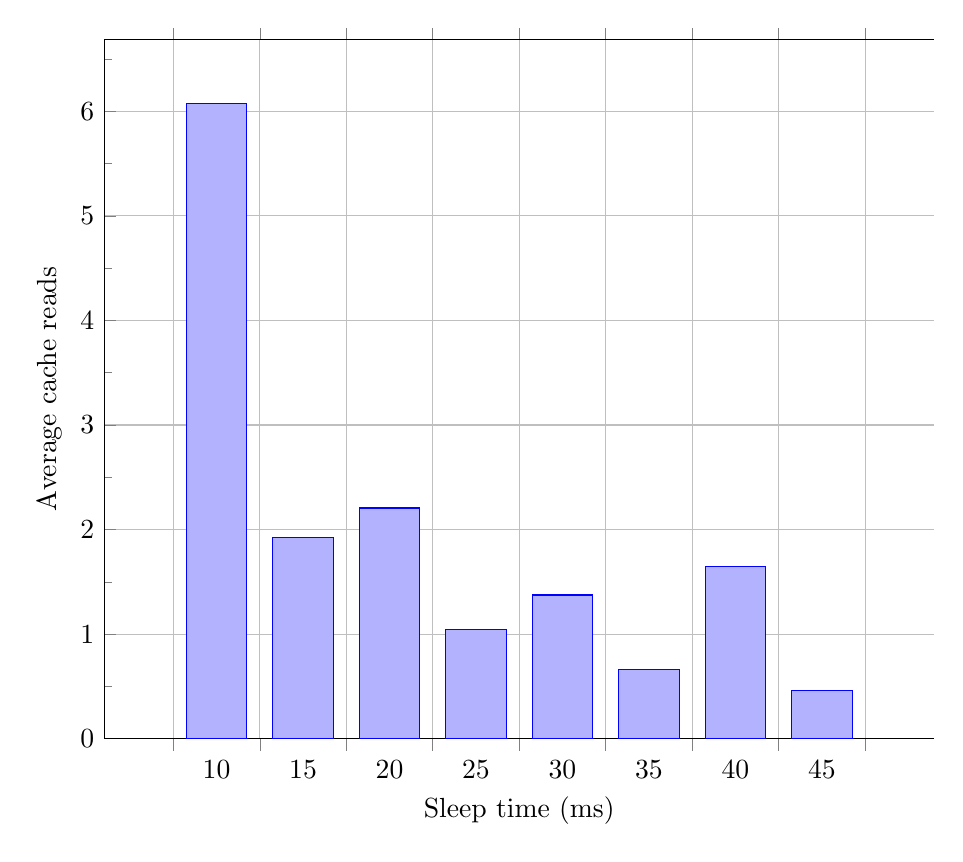
\begin{tikzpicture}
\begin{axis}
[
width=\resultsPlotWidthScale\textwidth,
axis y line*=left,
xlabel=Sleep time (ms),
ymin = 0,
%xmin = 0,
ylabel=Average cache reads,
%xtick={1, 2, 3, 4, 5, 6, 7, 8, 9},
%xticklabels={10, 15, 20, 25, 30, 35, 40, 45, 50},
%boxplot/draw direction=y,
%grid=both,
%ymajorgrids=true,
%yminorgrids=true,
ybar interval=0.7,
ymajorgrids=true,
%yminorgrids=true,
minor y tick num=1
%minor tick num=1
]
%\buildBoxPlot[black]{0}{0}{0}{0}{0}
%\buildBoxPlot[black]{0}{0}{0}{0}{0}
%\buildBoxPlot[black]{0}{0}{0}{0}{0}
%\buildBoxPlot[black]{0}{0}{0}{0}{0}
%\buildBoxPlot[black]{0}{0}{0}{0}{0}
%\buildBoxPlot[black]{0}{0}{0}{0}{0}
%\buildBoxPlot[black]{0}{0}{0}{0}{0}
%\buildBoxPlot[black]{0}{0}{0}{0}{0}
%\buildBoxPlot[black]{0}{0}{0}{0}{0}
\addplot coordinates {
	(10 ,6.076278918444858)
	(15 ,1.9250837336102817)
	(20 ,2.206446850393701)
	(25 ,1.044688862465319)
	(30 ,1.3747593094220163)
	(35 ,0.661782154722354)
	(40 ,1.6464805561590268)
	(45 ,0.46317152740208856)
	(50 ,1.858914282814271)
};

%matlab info
%     General model:
%     f(x) = (a/(x+b))+ c
%     Coefficients (with 95% confidence bounds):
%     a =       7.017  (-8.781, 22.82)
%     b =      -8.622  (-11.55, -5.697)
%     c =      0.9821  (0.01249, 1.952)
     
%\addplot[
%red,
%domain=10:50,
%samples=201,
%]
%{(7.017/(x-8.622))+ 0.9821};

\end{axis}
\end{tikzpicture}
	\caption{Decentralized solution with variable wait time cache reads experiment}
	\label{fig:exp:decen:sleep-cache}
\end{figure}

\Cref{fig:exp:decen:sleep-cache} show the average cache reads of the experiment.
A cache read only happens in the decentralized solution and is a consequence of the separation of receiving data in a separate thread.
The cache read happens if the wait time elapses before all turbine instances have responded with state information. The Number dos not include information of if the same turbine instance state has been read from cache multiple times.
The number of cache reads is declining. 
%, a fitted function of the plot has been put on top (red), the plot is in Matlab fitted against the function $\dfrac{a}{x + b} + c$.

\clearpage
\subsection{\nameref{subsec:Exper:perfom:2}}
The plots in this section relates to the second part of the \nameref{sec:Exper:perfom} experiment. In this graph the regulation cycle time is plotted against a variating number of turbines.

\begin{figure}[h!]
	\centering
	\begin{tikzpicture}
\begin{axis}
[
width=\textwidth,
axis y line*=left,
xlabel=Number of turbines,
ylabel=Regulation cycle time (ms),
ymin = 0,
xtick={1, 2, 3, 4, 5, 6, 7, 8, 9, 10, 11, 12, 13, 14, 15, 16, 17, 18, 19, 20},
xticklabels={5, 10, 15, 20, 25, 30, 35, 40, 45, 50, 55, 60, 65, 70, 75, 80, 85, 90, 95, 100},
boxplot/draw direction=y
]

%% /home/stefan/work/TestResults/Test5_Decentralized_success_12-4-2014_2100/nTurbines/DecentralizedLog0.csv
\buildBoxPlot{19.526002}{20.412002}{15.272001}{26.620001}{0.282}

%% /home/stefan/work/TestResults/Test5_Decentralized_success_12-4-2014_2100/nTurbines/DecentralizedLog1.csv
\buildBoxPlot{20.257002}{20.365001}{20.158001}{24.403002}{0.828002}

%% /home/stefan/work/TestResults/Test5_Decentralized_success_12-4-2014_2100/nTurbines/DecentralizedLog2.csv
\buildBoxPlot{20.221001}{20.311002}{20.126002}{24.641001}{3.778}

%% /home/stefan/work/TestResults/Test5_Decentralized_success_12-4-2014_2100/nTurbines/DecentralizedLog3.csv
\buildBoxPlot{20.203002}{20.321002}{20.066}{24.962}{0.246002}

%% /home/stefan/work/TestResults/Test5_Decentralized_success_12-4-2014_2100/nTurbines/DecentralizedLog4.csv
\buildBoxPlot{20.174001}{20.343}{19.946}{25.983002}{0.273002}

%% /home/stefan/work/TestResults/Test5_Decentralized_success_12-4-2014_2100/nTurbines/DecentralizedLog5.csv
\buildBoxPlot{20.190001}{20.286002}{20.051}{24.771001}{10.959001}

%% /home/stefan/work/TestResults/Test5_Decentralized_success_12-4-2014_2100/nTurbines/DecentralizedLog6.csv
\buildBoxPlot{20.079}{20.391001}{19.563001}{27.503001}{0.371002}

%% /home/stefan/work/TestResults/Test5_Decentralized_success_12-4-2014_2100/nTurbines/DecentralizedLog7.csv
\buildBoxPlot{20.176}{20.303001}{19.965}{30.63}{9.225}

%% /home/stefan/work/TestResults/Test5_Decentralized_success_12-4-2014_2100/nTurbines/DecentralizedLog8.csv
\buildBoxPlot{19.998}{20.351001}{19.215}{30.385002}{0.543001}

%% /home/stefan/work/TestResults/Test5_Decentralized_success_12-4-2014_2100/nTurbines/DecentralizedLog9.csv
\buildBoxPlot{20.008}{20.384001}{19.068001}{29.380001}{4.096002}

%% /home/stefan/work/TestResults/Test5_Decentralized_success_12-4-2014_2100/nTurbines/DecentralizedLog10.csv
\buildBoxPlot{19.902002}{20.353}{18.909001}{33.447001}{2.831002}

%% /home/stefan/work/TestResults/Test5_Decentralized_success_12-4-2014_2100/nTurbines/DecentralizedLog11.csv
\buildBoxPlot{19.937001}{20.373}{18.991001}{33.877001}{1.672002}

%% /home/stefan/work/TestResults/Test5_Decentralized_success_12-4-2014_2100/nTurbines/DecentralizedLog12.csv
\buildBoxPlot{20.056}{20.415001}{19.421002}{40.952001}{0.923001}

%% /home/stefan/work/TestResults/Test5_Decentralized_success_12-4-2014_2100/nTurbines/DecentralizedLog13.csv
\buildBoxPlot{20.215}{21.471}{19.378}{151.296001}{0.528001}

%% /home/stefan/work/TestResults/Test5_Decentralized_success_12-4-2014_2100/nTurbines/DecentralizedLog14.csv
\buildBoxPlot{19.920001}{20.535002}{18.897001}{53.699}{0.768}

%% /home/stefan/work/TestResults/Test5_Decentralized_success_12-4-2014_2100/nTurbines/DecentralizedLog15.csv
\buildBoxPlot{20.129002}{21.354002}{18.846002}{69.145001}{0.589001}

%% /home/stefan/work/TestResults/Test5_Decentralized_success_12-4-2014_2100/nTurbines/DecentralizedLog16.csv
\buildBoxPlot{20.189001}{22.247}{18.578001}{89.297001}{0.707}

%% /home/stefan/work/TestResults/Test5_Decentralized_success_12-4-2014_2100/nTurbines/DecentralizedLog17.csv
\buildBoxPlot{20.902001}{25.559001}{18.828}{142.836}{0.615001}

%% /home/stefan/work/TestResults/Test5_Decentralized_success_12-4-2014_2100/nTurbines/DecentralizedLog18.csv
\buildBoxPlot{25.609001}{35.368002}{20.078002}{150.034001}{0.579001}

%% /home/stefan/work/TestResults/Test5_Decentralized_success_12-4-2014_2100/nTurbines/DecentralizedLog19.csv
\buildBoxPlot{36.934001}{53.153001}{24.836001}{150.673002}{0.684001}


\addplot[thick, red!70] coordinates {
	(1 ,19.526002)
	(2 ,20.257002)
	(3 ,20.221001)
	(4 ,20.203002)
	(5 ,20.174001)
	(6 ,20.190001)
	(7 ,20.079)
	(8 ,20.176)
	(9 ,19.998)
	(10 ,20.008)
	(11 ,19.902002)
	(12 ,19.937001)
	(13 ,20.056)
	(14 ,20.215)
	(15 ,19.920001)
	(16 ,20.129002)
	(17 ,20.189001)
	(18 ,20.902001)
	(19 ,25.609001)
	(20 ,36.934001)
	
};

\end{axis}
\end{tikzpicture}
\begin{tikzpicture}
\begin{axis}
[
width=\textwidth,
axis y line*=left,
xlabel=Number of turbines,
ymin = 0,
ylabel=Average Cache hits,
xtick={1, 2, 3, 4, 5, 6, 7, 8, 9, 10, 11, 12, 13, 14, 15, 16, 17, 18, 19, 20},
xticklabels={5, 10, 15, 20, 25, 30, 35, 40, 45, 50, 55, 60, 65, 70, 75, 80, 85, 90, 95, 100},
boxplot/draw direction=y
]
\buildBoxPlot[black]{0}{0}{0}{0}{0}
\buildBoxPlot[black]{0}{0}{0}{0}{0}
\buildBoxPlot[black]{0}{0}{0}{0}{0}
\buildBoxPlot[black]{0}{0}{0}{0}{0}
\buildBoxPlot[black]{0}{0}{0}{0}{0}
\buildBoxPlot[black]{0}{0}{0}{0}{0}
\buildBoxPlot[black]{0}{0}{0}{0}{0}
\buildBoxPlot[black]{0}{0}{0}{0}{0}
\buildBoxPlot[black]{0}{0}{0}{0}{0}
\buildBoxPlot[black]{0}{0}{0}{0}{0}
\buildBoxPlot[black]{0}{0}{0}{0}{0}
\buildBoxPlot[black]{0}{0}{0}{0}{0}
\buildBoxPlot[black]{0}{0}{0}{0}{0}
\buildBoxPlot[black]{0}{0}{0}{0}{0}
\buildBoxPlot[black]{0}{0}{0}{0}{0}
\buildBoxPlot[black]{0}{0}{0}{0}{0}
\buildBoxPlot[black]{0}{0}{0}{0}{0}
\buildBoxPlot[black]{0}{0}{0}{0}{0}
\buildBoxPlot[black]{0}{0}{0}{0}{0}
\buildBoxPlot[black]{0}{0}{0}{0}{0}
\addplot[thick, orange!70] coordinates {
	(1 ,0.2591015249347438)
	(2 ,0.3423283799799435)
	(3 ,0.4286200856364344)
	(4 ,0.7913519050319182)
	(5 ,1.171919068056407)
	(6 ,0.4440826120490188)
	(7 ,1.8595523144717856)
	(8 ,0.506366007056297)
	(9 ,1.8951768000539848)
	(10 ,2.037951753081981)
	(11 ,2.0728170589196186)
	(12 ,2.0275369832294468)
	(13 ,1.2416290071090674)
	(14 ,3.5220372523313626)
	(15 ,2.115832267020478)
	(16 ,3.7417427229878832)
	(17 ,5.311682134712245)
	(18 ,8.473847137142263)
	(19 ,14.663734246038112)
	(20 ,22.06932793366117)
};
\end{axis}
\end{tikzpicture}
	\caption{Decentralized solution variable number of turbines experiment 1}
	\label{fig:exp:decen:turbines}
\end{figure}

\cref{fig:exp:decen:turbines} show regulation cycle time of the decentralized system compared with a variating number of turbines. The internal sleep parameter is fixed as 20~ms
It is seen the system performs with a constant regulation cycle time with 5 to 90 turbines, if only observing the median.
The quartiles are with the exception of the 5 turbines experiment of almost constant until 65, the same applies to the maximum values.
The extreme regulation cycle time values all  stop close to 150 ms.
At 70 turbines the maximum value sticks out notably it does look like a outlier however checking the raw data, it is not there are logged regulation cycle times for every ms value between it and the median.
It should be noted that all the data with a cycle time above 132~ms are collected from the same test machine.

\begin{figure}[h!]
	\centering
	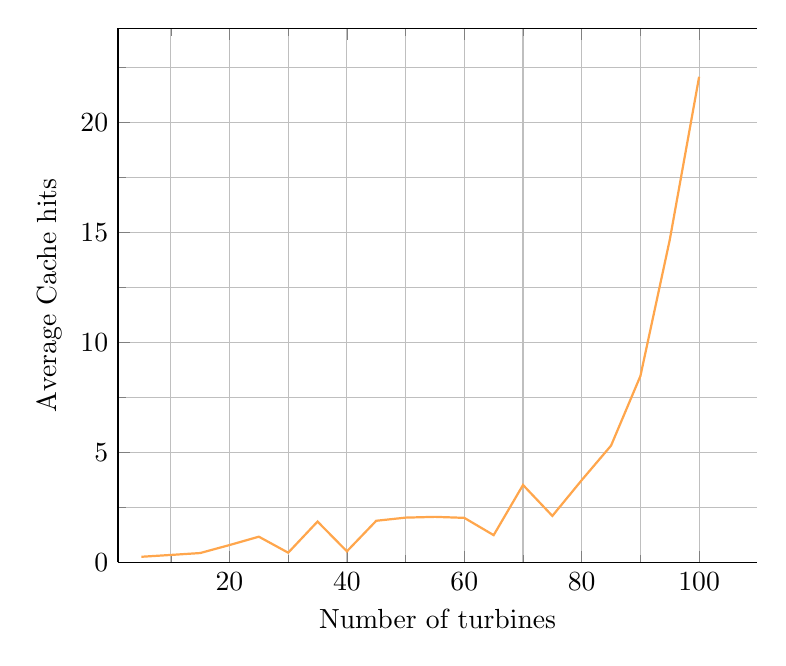
\begin{tikzpicture}
\begin{axis}
[
width=\resultsFigureWidthScale\textwidth,
axis y line*=left,
xlabel=Number of turbines,
ymin = 0,
xmin = 1,
ylabel=Average Cache hits,
%xtick={1, 2, 3, 4, 5, 6, 7, 8, 9, 10, 11, 12, 13, 14, 15, 16, 17, 18, 19, 20},
%xticklabels={5, 10, 15, 20, 25, 30, 35, 40, 45, 50, 55, 60, 65, 70, 75, 80, 85, 90, 95, 100},
%boxplot/draw direction=y,
grid=both,
minor tick num=1
]
%\buildBoxPlot[black]{0}{0}{0}{0}{0}
%\buildBoxPlot[black]{0}{0}{0}{0}{0}
%\buildBoxPlot[black]{0}{0}{0}{0}{0}
%\buildBoxPlot[black]{0}{0}{0}{0}{0}
%\buildBoxPlot[black]{0}{0}{0}{0}{0}
%\buildBoxPlot[black]{0}{0}{0}{0}{0}
%\buildBoxPlot[black]{0}{0}{0}{0}{0}
%\buildBoxPlot[black]{0}{0}{0}{0}{0}
%\buildBoxPlot[black]{0}{0}{0}{0}{0}
%\buildBoxPlot[black]{0}{0}{0}{0}{0}
%\buildBoxPlot[black]{0}{0}{0}{0}{0}
%\buildBoxPlot[black]{0}{0}{0}{0}{0}
%\buildBoxPlot[black]{0}{0}{0}{0}{0}
%\buildBoxPlot[black]{0}{0}{0}{0}{0}
%\buildBoxPlot[black]{0}{0}{0}{0}{0}
%\buildBoxPlot[black]{0}{0}{0}{0}{0}
%\buildBoxPlot[black]{0}{0}{0}{0}{0}
%\buildBoxPlot[black]{0}{0}{0}{0}{0}
%\buildBoxPlot[black]{0}{0}{0}{0}{0}
%\buildBoxPlot[black]{0}{0}{0}{0}{0}
\addplot[thick, orange!70] coordinates {
	(5 ,0.2591015249347438)
	(10 ,0.3423283799799435)
	(15 ,0.4286200856364344)
	(20 ,0.7913519050319182)
	(25 ,1.171919068056407)
	(30 ,0.4440826120490188)
	(35 ,1.8595523144717856)
	(40 ,0.506366007056297)
	(45 ,1.8951768000539848)
	(50 ,2.037951753081981)
	(55 ,2.0728170589196186)
	(60 ,2.0275369832294468)
	(65 ,1.2416290071090674)
	(70 ,3.5220372523313626)
	(75 ,2.115832267020478)
	(80 ,3.7417427229878832)
	(85 ,5.311682134712245)
	(90 ,8.473847137142263)
	(95 ,14.663734246038112)
	(100 ,22.06932793366117)
};
\end{axis}
\end{tikzpicture}
	\caption{Decentralized solution variable number of turbines experiment 1}
	\label{fig:exp:decen:turbines_cache}
\end{figure}


\cref{fig:exp:decen:turbines_cache} show the amount of cache reads the simulation had during part 2 of the experiment.
The plot almost lines up with a exponential curve. Also \cref{fig:exp:decen:turbines,fig:exp:decen:turbines_cache} seams to suddenly increase around 65 ms.
\clearpage
\section{\ref{PS:Q:Scalability}}\FloatBarrier

\begin{figure}[h!]
	\centering
	\begin{tikzpicture}
\begin{axis}
[
	width=\resultsPlotWidthScale\textwidth,
	axis y line*=left,
	xlabel=Number of turbines,
	ylabel=Regulation cycle time (ms),
	ymin = 0,
	xmin = 1, xmax = 20,
	xtick={1, 2, 3, 4, 5, 6, 7, 8, 9, 10, 11, 12, 13, 14, 15, 16, 17, 18, 19},
	xticklabels={ , , 15, , 25, , 35, , 45, , 55, , 65, , 75, , 85, , 95},
%	xticklabels={5, 10, 15, 20, 25, 30, 35, 40, 45, 50, 55, 60, 65, 70, 75, 80, 85, 90, 95},
	boxplot/draw direction=y,
	ymajorgrids=true,
	yminorgrids=true,
%	minor y tick num=1,
	max space between ticks=17.5
]

%% /home/stefan/work/TestResults/Test4_Centralized_success_12-4-2014_2024/CentralizedLog2.csv
%\buildBoxPlot{0.871522}{0.955}{0.809034}{12.535623}{0.541744}
\buildBoxPlot[black]{0}{0}{0}{0}{0}

%% /home/stefan/work/TestResults/Test4_Centralized_success_12-4-2014_2024/CentralizedLog3.csv
\buildBoxPlot{1.168815}{1.310873}{1.081427}{24.566027}{0.591135}

%% /home/stefan/work/TestResults/Test4_Centralized_success_12-4-2014_2024/CentralizedLog4.csv
\buildBoxPlot{1.398871}{1.613768}{1.303639}{19.188073}{0.747894}

%% /home/stefan/work/TestResults/Test4_Centralized_success_12-4-2014_2024/CentralizedLog5.csv
\buildBoxPlot{1.722236}{1.981776}{1.596331}{13.257023}{1.077214}

%% /home/stefan/work/TestResults/Test4_Centralized_success_12-4-2014_2024/CentralizedLog6.csv
\buildBoxPlot{1.978881}{2.337657}{1.823133}{20.243534}{1.278172}

%% /home/stefan/work/TestResults/Test4_Centralized_success_12-4-2014_2024/CentralizedLog7.csv
\buildBoxPlot{2.985681}{3.527133}{2.724617}{102.89112}{1.917354}

%% /home/stefan/work/TestResults/Test4_Centralized_success_12-4-2014_2024/CentralizedLog8.csv
\buildBoxPlot{5.662268}{6.776311}{5.315074}{55.800126}{3.845115}

%% /home/stefan/work/TestResults/Test4_Centralized_success_12-4-2014_2024/CentralizedLog9.csv
\buildBoxPlot{14.607313}{22.842589}{10.21933}{40.119104}{7.578863}

%% /home/stefan/work/TestResults/Test4_Centralized_success_12-4-2014_2024/CentralizedLog10.csv
\buildBoxPlot{16.673738}{25.382756}{14.810635}{46.844742}{12.042462}

%% /home/stefan/work/TestResults/Test4_Centralized_success_12-4-2014_2024/CentralizedLog11.csv
\buildBoxPlot{20.220936}{27.962488}{19.190067}{63.348974}{17.058657}

%% /home/stefan/work/TestResults/Test4_Centralized_success_12-4-2014_2024/CentralizedLog12.csv
\buildBoxPlot{31.587407}{33.177592}{24.950794}{46.841843}{22.941051}

%% /home/stefan/work/TestResults/Test4_Centralized_success_12-4-2014_2024/CentralizedLog13.csv
\buildBoxPlot{36.93711}{38.790125}{32.230331}{51.398495}{29.702809}

%% /home/stefan/work/TestResults/Test4_Centralized_success_12-4-2014_2024/CentralizedLog14.csv
\buildBoxPlot{40.231022}{42.885333}{36.673407}{77.051599}{33.854906}

%% /home/stefan/work/TestResults/Test4_Centralized_success_12-4-2014_2024/CentralizedLog15.csv
\buildBoxPlot{45.380062}{48.694656}{42.841453}{225.894089}{39.402015}

%% /home/stefan/work/TestResults/Test4_Centralized_success_12-4-2014_2024/CentralizedLog16.csv
\buildBoxPlot{51.425649}{54.462315}{48.438981}{250.200229}{45.062697}

%% /home/stefan/work/TestResults/Test4_Centralized_success_12-4-2014_2024/CentralizedLog17.csv
\buildBoxPlot{58.196177}{62.557505}{55.582236}{271.626595}{51.598593}

%% /home/stefan/work/TestResults/Test4_Centralized_success_12-4-2014_2024/CentralizedLog18.csv
\buildBoxPlot{64.70376}{70.553035}{62.053219}{278.866888}{57.401402}

%% /home/stefan/work/TestResults/Test4_Centralized_success_12-4-2014_2024/CentralizedLog19.csv
\buildBoxPlot{73.715686}{80.566923}{69.809765}{287.542878}{65.698499}

%% /home/stefan/work/TestResults/Test4_Centralized_success_12-4-2014_2024/CentralizedLog20.csv
\buildBoxPlot{82.961949}{151.608592}{77.825807}{290.243704}{72.589561}


\addplot[thick, red!70] coordinates {
%	(1 ,0.871522)
	(2 ,1.168815)
	(3 ,1.398871)
	(4 ,1.722236)
	(5 ,1.978881)
	(6 ,2.985681)
	(7 ,5.662268)
	(8 ,14.607313)
	(9 ,16.673738)
	(10 ,20.220936)
	(11 ,31.587407)
	(12 ,36.93711)
	(13 ,40.231022)
	(14 ,45.380062)
	(15 ,51.425649)
	(16 ,58.196177)
	(17 ,64.70376)
	(18 ,73.715686)
	(19 ,82.961949)
};

\end{axis}
\end{tikzpicture}

	\caption{Centralized solution variable number of turbines experiment 1}
	\label{fig:exp:cen:turbines}
\end{figure}

The \nameref{subsec:Exper:Scale} experiment results are described in this section, these experiments are done against the centralized solution. \Cref{fig:exp:cen:turbines} show the comparison experiment done with the centralized solution. The median values initially are constant, this is from 10 turbines to 30 turbines, from 35 and up the median is linearly increasing.
From 70 Turbines the regulation start to have larger max values which increases linearly as well.








